\documentclass[titlepage]{jsarticle}
\usepackage[dvipdfmx]{graphicx}
\usepackage{listings}
\usepackage{cprotect}
\usepackage{comment}
\usepackage{h31ec-exp}
\lstset{
    basicstyle={\ttfamily},
    identifierstyle={\small},
    commentstyle={\smallitshape},
    keywordstyle={\small\bfseries},
    ndkeywordstyle={\small},
    stringstyle={\small\ttfamily},
    frame={tb},
    breaklines=true,
    columns=[l]{fullflexible},
    numbers=left,
    xrightmargin=0zw,
    xleftmargin=3zw,
    numberstyle={\scriptsize},
    stepnumber=1,
    numbersep=1zw,
    lineskip=-0.5ex,
    keepspaces=true,
    language=c
}
\renewcommand{\lstlistingname}{リスト}
\makeatletter
\newcommand{\figcaption}[1]{\def\@captype{figure}\caption{#1}}
\newcommand{\tblcaption}[1]{\def\@captype{table}\caption{#1}}
\makeatother

\title{信号処理プログラミング}
\grade{4年32番}
\author{平田 蓮}
\team{}
\date{2020年8月7日}
\expdate{2020年5月21日, 5月28日, 6月4日, 6月11日}
\coauthor{}

\begin{document}
\maketitle
\section{目的}
    アナログ信号をディジタルデータに変換し, ディジタル機器で処理するために必要な基礎事項について学習し,
    C言語で基本的な信号処理プログラムを作成する.
    また音声フォーマットの一つであるWAVEファイルの構造を理解し, 音声データの入出力プログラムを作成する.

\section{周期関数の生成と可視化}
    正弦波のように一定周期ごとに同じ波形が繰り返される関数を\textbf{周期関数}と呼ぶ.
    よく知られている周期関数として, のこぎり波などがある.
    本節では周期関数に関する演習を行う.

    \paragraph{演習1-3} 任意の孤度$r$に対して, 矩形波の振幅値を求める関数\verb|squ|を作成せよ.

        作成した関数をリスト\ref{src:squ}に示す.

        \begin{lstlisting}[caption=squ.c, label=src:squ]
double squ(double r) {
    return rad(r) < PI ? 1 : -1;
}\end{lstlisting}

        与えられた孤度$r$を演習1-1で実装した\verb|rad|を使い$[0:2\pi]$の範囲に変換する.
        その孤度が$\pi$未満の場合に1を返し, それ以外の場合は-1を返すことで矩形波を出力できた.

        図\ref{fig:squ}に横軸に$r$, 縦軸に\verb|rad(r)|を取ったグラフを示す.
        図より, 矩形波が正しく出力できていることがわかる.

        \begin{figure}[h]
            \centering
            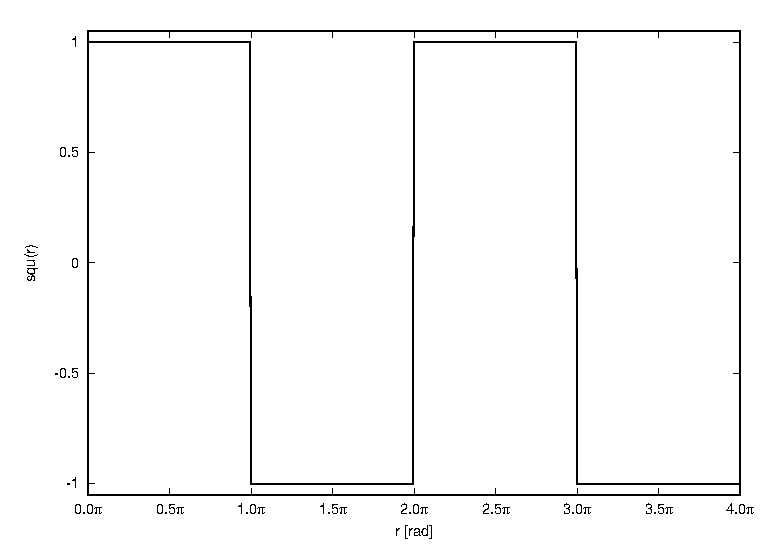
\includegraphics[width=0.8\hsize]{images/squ.eps}
            \cprotect\caption{\verb|squ|による矩形波}
            \label{fig:squ}
        \end{figure}

    \paragraph{演習1-4} 任意の孤度$r$に対して, 三角波の振幅値を求める関数\verb|tri|を作成せよ.

        作成した関数をリスト\ref{src:tri}に示す.

        \begin{lstlisting}[caption=tri.c, label=src:tri]
double tri(double r) {
    r += PI / 2.0;
    if (rad(r) < PI) {
        return 2.0 * rad(r) / PI - 1.0;
    } else {
        return 2.0 - 2.0 * (rad(r) - PI / 2.0) / PI;
    }
}\end{lstlisting}

        与えられた孤度$r$を演習1-1で実装した\verb|rad|を使い$[0:2\pi)$の範囲に変換する.
        その後, $r$の位相を変化させた後, 区間$[0:\pi), [\pi:2\pi)$に分けて処理を行っている.

        図\ref{fig:tri}に横軸に$r$, 縦軸に\verb|tri(r)|を取ったグラフを示す.
        図より, 三角波が正しく出力できていることがわかる.

        \begin{figure}[h]
            \centering
            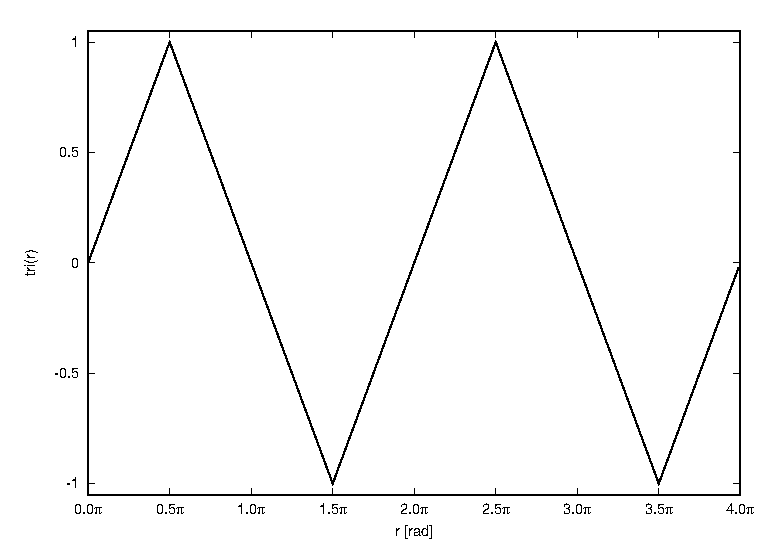
\includegraphics[width=0.8\hsize]{images/tri.eps}
            \cprotect\caption{\verb|tri|による三角波}
            \label{fig:tri}
        \end{figure}

\section{サンプリング}
    アナログ信号波形をディジタルデータに変換する手法に\textbf{サンプリング}がある.
    本節では演習問題を通して実際にサンプリングの様子を観察する.

    \paragraph{演習2-3} 量子化誤差を評価するため, sin10af1.cに量子化における
    2乗平均平方根誤差を計算する機能を追加せよ.

        sin10af1.cに追加した部分を抜粋してリスト\ref{src:rms}に示す.
        

        \begin{lstlisting}[caption=sin10af1.c, label=src:rms]
#define DT 10
#define TEND 1000

int main(int argc, char **argv) {
    int t;
    double vin, esum = 0, rms;
    unsigned char vout;

    for (t = 0; t <= TEND; t += DT) {
        esum += (vin - vout) * (vin - vout);
    }

    rms = sqrt(esum / (TEND / DT + 1));
    printf("#E_RMS: %f\n", rms);
}\end{lstlisting}

        上のプログラムを使用して振幅100, 周波数4 Hzの正弦波をサンプリングしたときのRMS誤差を求めると,
        約0.559であった.

    \paragraph{演習2-4} 各時刻の振幅値の小数点以下第1位を四捨五入して量子化するプログラムsin10af2.cを作成し,
    量子化によるRMS誤差の軽減効果を定量的に調べよ.

        作成したプログラムを一部抜粋してリスト\ref{src:rms2}に示す.

        \begin{lstlisting}[caption=sin10af2.c, label=src:rms2]
#define DT 10
#define TEND 1000

int main(int argc, char **argv) {
    int t;
    double vin, esum = 0, rms;
    unsigned char vout;

    for (t = 0; t <= TEND; t += DT) {
        if (vin > 255) {
            vout = 255;
        } else if (vin < 0) {
            vout = 0;
        } else {
            vout = vin + 0.5;
        }

        esum += (vin - vout) * (vin - vout);
    }

    rms = sqrt(esum / (TEND / DT + 1));
    printf("#E_RMS: %f\n", rms);
}\end{lstlisting}

        15行目で, sin10af1.cでは\verb|vout = vin|としていたところを,
        0.5を足すことで整数値に直されるときに四捨五入されることになる.

        このプログラムを使用して演習2-3を同じように振幅100, 周波数4 Hzの正弦波をサンプリングした時のRMS誤差を求めると,
        約0.293であった.

        四捨五入をしなかった場合と比べると,約0.266の差があることがわかり,
        四捨五入をすることにRMS誤差の軽減効果が大きくあることがわかる.

    \paragraph{演習2-6} 正弦波の振幅, 周波数, 位相, 標本化間隔をコマンドライン引数で指定した時,
    サンプリング結果を出力するプログラムsinafpt.cを作成せよ.

        作成したプログラムをリスト\ref{src:sinafpt}に一部抜粋して示す.
        ここで, 正弦波の位相はrad単位の実数で指定することとした.

        \begin{lstlisting}[caption=sinafpt.c, label=src:sinafpt]
#define BIAS 0x80
#define TEND 1000

int main(int argc, char **argv) {
    int t;
    double amp, frq, smp, phf, r, vin;
    unsigned char vout;

    for (t = 0; t <= TEND; t += smp) {
        r = t / 1000.0 * 2.0 * PI * frq + phf;
        vin = amp * sin(r) + BIAS;
        if (vin > 255) {
            vout = 255;
        } else if (vin < 0) {
            vout = 0;
        } else {
            vout = vin + 0.5;
        }

        printf("%d, %4d\n", t, vout);
    }
}\end{lstlisting}

        このプログラムを使用して, 振幅100, 周波数5 Hz,
        位相1.57 rad ($\displaystyle\approx \frac{\pi}{2}$ [rad]),
        標本化間隔5 msの正弦波をサンプリングした結果を図\ref{fig:sinafpt}に示す.
        図より, 正しくサンプリングされていることがわかる.

        \begin{figure}[h]
            \centering
            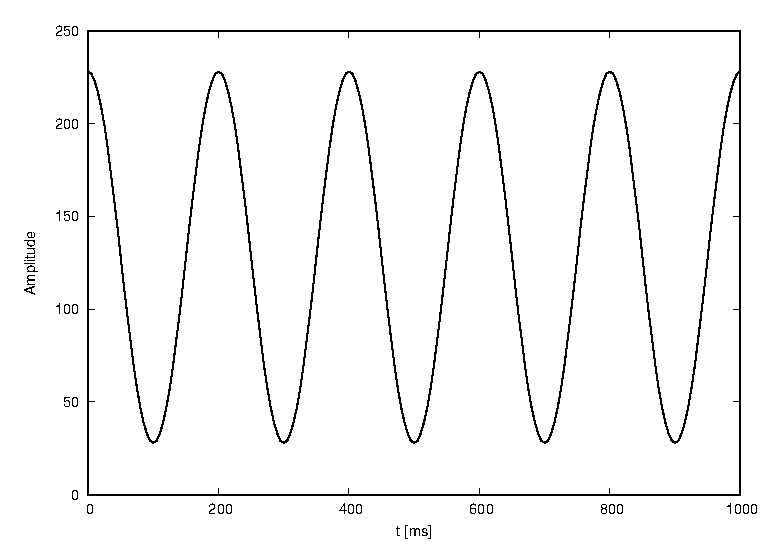
\includegraphics[width=0.8\hsize]{images/sin.eps}
            \caption{振幅100, 周波数5 Hz, 位相1.57 radの正弦波}
            \label{fig:sinafpt}
        \end{figure}
    
    \paragraph{演習2-7} 振幅, 周波数, 標本化間隔をコマンドライン引数で指定したとき,
    のこぎり波, 矩形波, 三角波を出力するプログラムXXXaft.cを作成せよ.
    (XXXはのこぎり波はsaw, 矩形波はsqu, 三角波はtri)

        作成したプログラムを一部抜粋してリスト\ref{src:sawaft}, \ref{src:squaft}, \ref{src:triaft}に示す.

        \begin{lstlisting}[caption=sawaft.c, label=src:sawaft]
double rad(double r) {
    if (r >= 0) {
        return fmod(r, 2 * PI);
    } else {
        return 2 * PI - fmod(-r, 2 * PI);
    }
}

double saw(double r) {
    return 1 - rad(r) / PI;
}

int main(int argc, char **argv) {
    int t;
    double r, amp, frq, smp, vin, vout;

    amp = atof(argv[1]);
    frq = atof(argv[2]);
    smp = atof(argv[3]);

    for (t = 0; t <= 1000; t += smp) {
        r = t / 1000.0 * 2.0 * PI * frq;
        vin = amp * saw(r);
        vout = vin;
        printf("%d, %4f\n", t, vout);
    }
}\end{lstlisting}

        \begin{lstlisting}[caption=squaft.c, label=src:squaft]
double rad(double r) {
    if (r >= 0) {
        return fmod(r, 2 * PI);
    } else {
        return 2 * PI - fmod(-r, 2 * PI);
    }
}

double squ(double r) {
    return rad(r) < PI ? 1 : -1;
}

int main(int argc, char **argv) {
    int t;
    double r, amp, frq, smp, vin, vout;

    amp = atof(argv[1]);
    frq = atof(argv[2]);
    smp = atof(argv[3]);

    for (t = 0; t <= 1000; t += smp) {
        r = t / 1000.0 * 2.0 * PI * frq;
        vin = amp * squ(r);
        vout = vin;
        printf("%d, %4f\n", t, vout);
    }
}\end{lstlisting}

        \begin{lstlisting}[caption=triaft.c, label=src:triaft]
double rad(double r) {
    if (r >= 0) {
        return fmod(r, 2 * PI);
    } else {
        return 2 * PI - fmod(-r, 2 * PI);
    }
}

double tri(double r) {
    r += PI / 2.0;
    if (rad(r) < PI) {
        return 2.0 * rad(r) / PI - 1.0;
    } else {
        return 2.0 - 2.0 * (rad(r) - PI / 2.0) / PI;
    }
}

int main(int argc, char **argv) {
    int t;
    double r, amp, frq, smp, vin, vout;

    amp = atof(argv[1]);
    frq = atof(argv[2]);
    smp = atof(argv[3]);

    for (t = 0; t <= 1000; t += smp) {
        r = t / 1000.0 * 2.0 * PI * frq;
        vin = amp * tri(r);
        vout = vin;
        printf("%d, %4f\n", t, vout);
    }
}\end{lstlisting}

        これらのプログラムを使って振幅2.5, 周波数3 Hz, 標本化間隔5 msののこぎり波, 矩形波, 三角波を
        サンプリングしたものを図\ref{fig:sawaft}, \ref{fig:squaft}, \ref{fig:triaft}に示す.

        \begin{figure}[h]
            \centering
            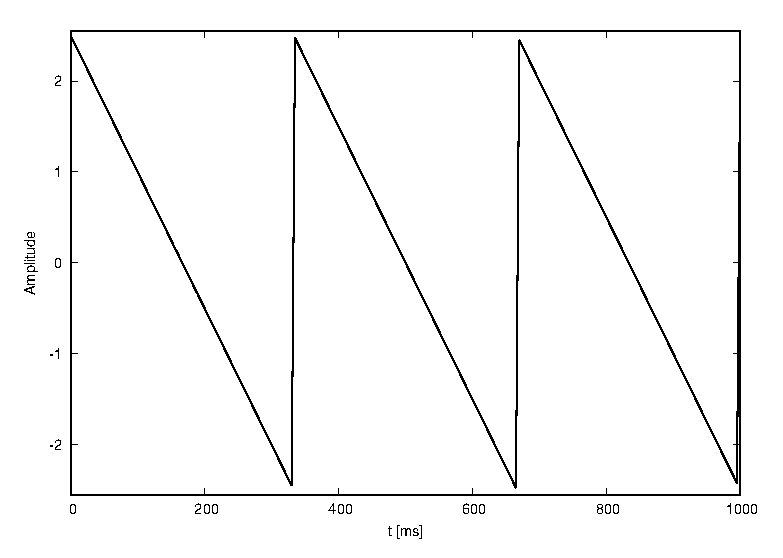
\includegraphics[width=0.8\hsize]{images/sawaft.eps}
            \caption{振幅2.5, 周波数3 Hz, 標本化間隔5 msののこぎり波}
            \label{fig:sawaft}
        \end{figure}

        \begin{figure}[h]
            \centering
            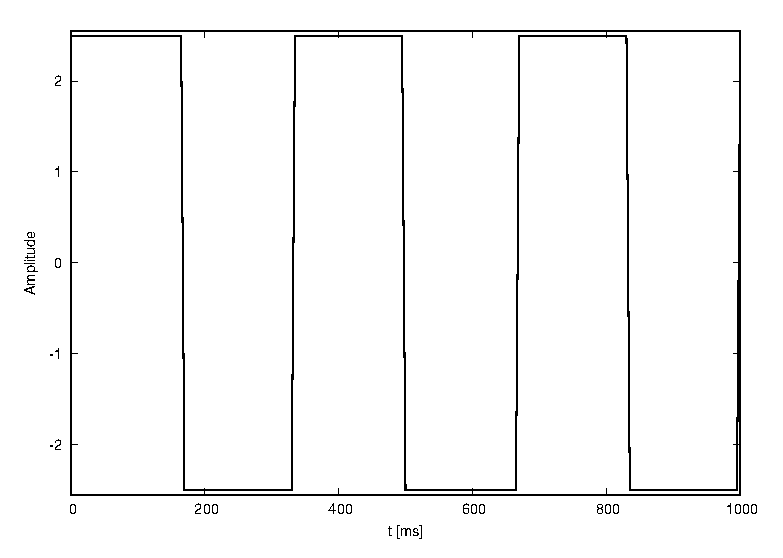
\includegraphics[width=0.8\hsize]{images/squaft.eps}
            \caption{振幅2.5, 周波数3 Hz, 標本化間隔5 msの矩形波}
            \label{fig:squaft}
        \end{figure}

        \begin{figure}[h]
            \centering
            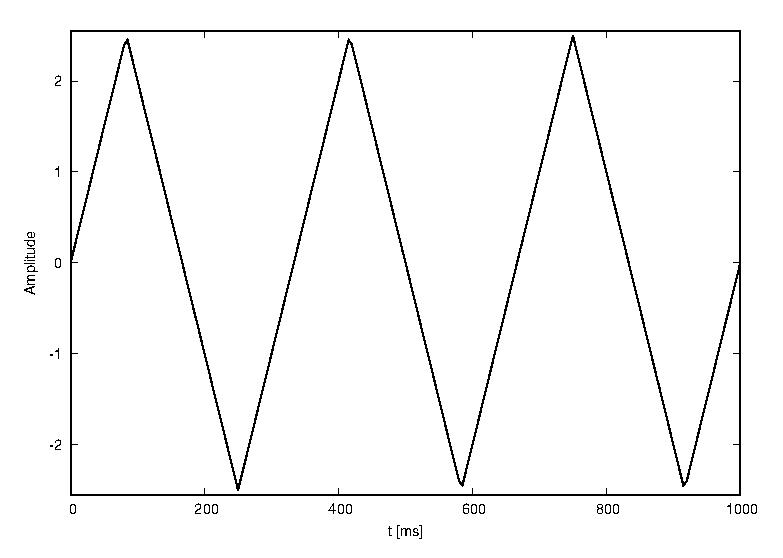
\includegraphics[width=0.8\hsize]{images/triaft.eps}
            \caption{振幅2.5, 周波数3 Hz, 標本化間隔5 msの三角波}
            \label{fig:triaft}
        \end{figure}

        図から, 正しくサンプリングできていることがわかる.

\section{信号処理プログラムの分類}
    信号処理プログラムは, オンライン型をオフライン型の二種類に分類することができる.
    データを一つ取り込むたびに\textbf{逐次処理}を行うオンライン型に対して,
    オフライン型はデータを一定数取り込んだ後に\textbf{一括処理}を行う.

\section{雑音除去}
    信号に重畳された雑音を取り除く処理は, 極めて基本的な信号処理である.
    演習3では雑音の処理に関する演習を行う.

    \paragraph{演習3-3} 5点単純移動平均プログラムmvave5-?.cを作成せよ (?はオンライン型は1, オフライン型は2).

        作成したプログラムをリスト\ref{src:mvave5-1}, \ref{src:mvave5-2}に抜粋して示す.

        \begin{lstlisting}[caption=mvave5-1.c, label=src:mvave5-1]
#define BUFSIZE 80
#define ROUND(x) ((x > 0) ? (x + 0.5) : (x - 0.5))

#define POINTS 5

int main(int argc, char **argv) {
    int tm[(POINTS + 1) / 2] = {}, amp[POINTS] = {}, sum = 0, pt1 = 0, pt2 = 0;
    char buf[BUFSIZE];
    unsigned char vout;
    FILE *fp;

    while (fgets(buf, sizeof(buf), fp) != NULL) {
        if (buf[0] == '#') continue;

        sum -= amp[pt1];
        
        tm[pt2]  = atoi(strtok(buf, ","));
        amp[pt1] = atoi(strtok(NULL, "\r\n\0"));

        sum += amp[pt1];

        pt1 = (pt1 + 1) % POINTS;
        pt2 = (pt2 + 1) % ((POINTS + 1) / 2);

        if (amp[pt1] == 0) continue;

        vout = ROUND(sum / (double)POINTS);
        printf("%d, %4d\n", tm[pt2], vout);
    }
}\end{lstlisting}

        \begin{lstlisting}[caption=mvave5-2.c, label=src:mvave5-2]
#define BUFSIZE 80
#define DATANUM 1000
#define ROUND(x) ((x > 0) ? (x + 0.5) : (x - 0.5))

#define POINTS 5

int main(int argc, char **argv) {
    int tm[DATANUM], amp[DATANUM], sum = 0, n, data_num;
    char buf[BUFSIZE];
    unsigned char vout;
    FILE *fp;

    for (n = 0; n < DATANUM; n++) {
        if (fgets(buf, sizeof(buf), fp) == NULL) break;
        if (buf[0] == '#') continue;
        tm[n]  = atoi(strtok(buf, ","));
        amp[n] = atoi(strtok(NULL, "\r\n\0"));
    }
    fclose(fp);

    data_num = n;

    for (int n = 0; n < data_num; n++) {
        sum += amp[n];

        if (n < POINTS - 1) continue;
        if (n >= POINTS) sum -= amp[n - POINTS];

        vout = ROUND(sum / (double)POINTS);

        printf("%d, %4d\n", tm[n - POINTS / 2], vout);
    }
}\end{lstlisting}

        それぞれ, \verb|POINTS|の値を$N$にすることで$N$点単純移動平均プログラムとすることができる.
        直近5つのデータと2つの時刻を利用することで平均を求める際の計算量を軽減することができた.

        これらのプログラムで, 振幅100, 周波数4 Hzの正弦波に演習3-1で実装したadd-wn2.cを使用して最大振幅10の
        白色雑音を加えた波形に雑音除去を行った波形を図\ref{fig:mvave1}, \ref{fig:mvave2}に示す.

        \begin{figure}[h]
            \centering
            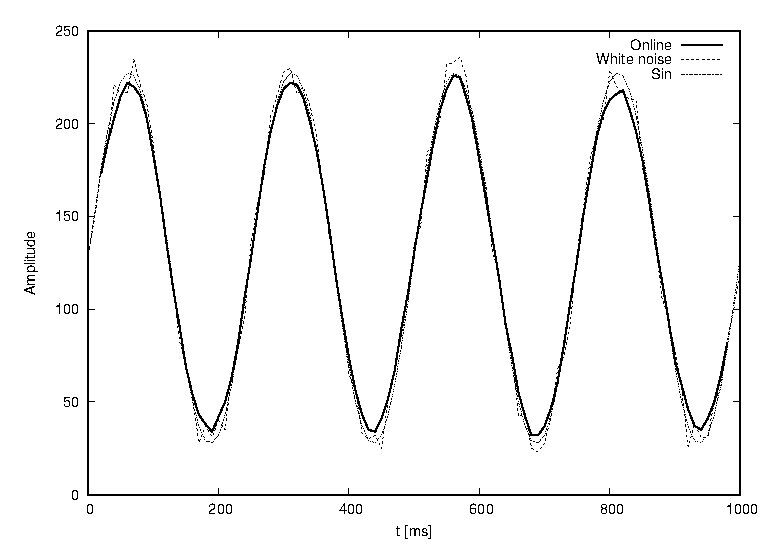
\includegraphics[width=0.8\hsize]{images/mvave5-1.eps}
            \caption{オンライン型プログラムを利用して雑音を取り除いた波形}
            \label{fig:mvave1}
        \end{figure}

        \begin{figure}[h]
            \centering
            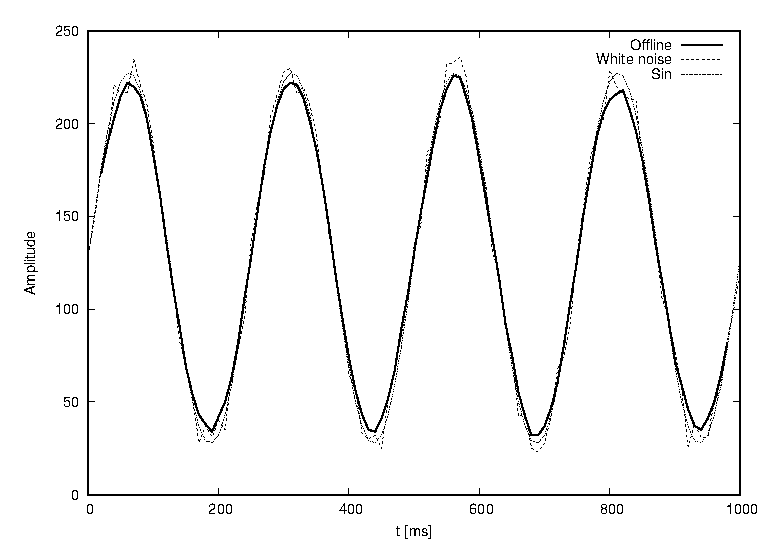
\includegraphics[width=0.8\hsize]{images/mvave5-2.eps}
            \caption{オフライン型プログラムを利用して雑音を取り除いた波形}
            \label{fig:mvave2}
        \end{figure}

        図から, どちらの波形も元の波形に近づいていることがわかる.
        また, 5点平均を取っているため, データの始点と終点がそれぞれ2つずつ欠けている.

\section{時系列データの解析}
    周期的なアナログ信号$x(t)$に由来する時系列データ$x_i;i=1,2,\dots,N$が与えられたとき,
    元の信号の基本周波数, 振幅, 位相などを求めることを信号解析を呼ぶ.
    本実験では信号の\textbf{最小値}, \textbf{最大値}, \textbf{平均値}, \textbf{標準偏差}, \textbf{最大振幅}, \textbf{実効値}を求める.

    \paragraph{演習4-3} 参考文献\cite{Text}のリスト5を完成させよ.
    次に, コマンドライン引数として指定された2つのCSVファイルについてファイルについて,
    時系列データの差を取るオフライン型プログラムdiff2.cを作成せよ.

        作成したプログラムを一部抜粋してリスト\ref{src:diff}に示す.
        
        \begin{lstlisting}[caption=diff2.c, label=src:diff]
#define BUFSIZE 80
#define DATANUM 1000

int main(int argc, char **argv) {
    int tm1[DATANUM] = {}, tm2[DATANUM] = {}, amp1[DATANUM], amp2[DATANUM], dif, n, m;
    char buf[BUFSIZE];

    char *p;
    FILE *fp1, *fp2;

    for (n = 0; n <= DATANUM; n++) {
        if (fgets(buf, sizeof(buf), fp1) == NULL) break;
        if (buf[0] == '#') continue;
        tm1[n]  = atoi(strtok(buf, ","));
        amp1[n] = atof(strtok(NULL, "\r\n\0"));
    }
    fclose(fp1);

    for (n = 0; n <= DATANUM; n++) {
        if (fgets(buf, sizeof(buf), fp2) == NULL) break;
        if (buf[0] == '#') continue;
        tm2[n]  = atoi(strtok(buf, ","));
        amp2[n] = atoi(strtok(NULL, "\r\n\0"));
    }
    fclose(fp2);

    for (n = m = 0; n < DATANUM; n++) {
        while (tm2[m] < tm1[n]) m++;
        while (tm1[n] < tm2[m]) n++;

        if (tm1[n] != tm2[m]) continue;

        dif = amp1[n] - amp2[m];
        printf("%d, %4d\n", tm1[n], dif);
    }
}\end{lstlisting}

        はじめに2つのデータを読み込み, その後に同時刻のデータの差をとるオフライン処理をしている.

        このプログラムを使用して振幅100, 周波数4 Hzの正弦波とそれに最大振幅10の白色雑音を加えた波の差を
        取ったデータを図\ref{fig:diff}に示す.

        \begin{figure}[h]
            \centering
            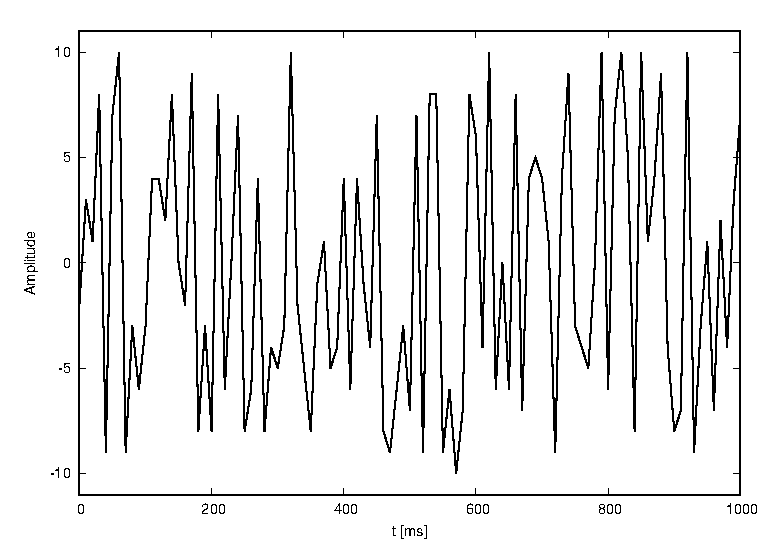
\includegraphics[width=0.8\hsize]{images/diff.eps}
            \caption{最大振幅10の白色雑音}
            \label{fig:diff}
        \end{figure}

        図より, 正しく最大振幅10の白色雑音が取り出せていることがわかる.

    \paragraph{演習4-4} 元信号のCSVファイルを第1引数, 雑音が重畳されたCSVファイルを第2引数として与えられたときに,
    SNR[dB]を求めるプログラムsnr.cを作成せよ. このプログラムを使って,
    元信号が正弦波の場合について, 3点移動平均と5点移動平均の雑音除去性能を定量的に比較せよ.
        
        作成したプログラムを一部抜粋してリスト\ref{src:snr}に示す.

        \begin{lstlisting}[caption=snr.c, label=src:snr]
#define BIAS 0x80
#define BUFSIZE 80
#define DATANUM 1000

int main(int argc, char **argv) {
    int tm1[DATANUM] = {}, tm2, amp1[DATANUM], amp2, n, sum1 = 0, sum2 = 0;
    char buf[BUFSIZE];

    FILE *fp1, *fp2;

    for (n = 0; n <= DATANUM; n++) {
        if (fgets(buf, sizeof(buf), fp1) == NULL) break;
        if (buf[0] == '#') continue;
        tm1[n]  = atoi(strtok(buf, ","));
        amp1[n] = atof(strtok(NULL, "\r\n\0"));

        sum1 += (amp1[n] - BIAS) * (amp1[n] - BIAS);
    }
    fclose(fp1);

    for (n = 0; n <= DATANUM; n++) {
        if (fgets(buf, sizeof(buf), fp2) == NULL) break;
        if (buf[0] == '#') continue;
        tm2  = atoi(strtok(buf, ","));
        amp2 = atoi(strtok(NULL, "\r\n\0"));

        sum2 += (amp2 - amp1[n]) * (amp2 - amp1[n]);
    }
    fclose(fp2);

    printf("SNR[dB]: %f\n", 10 * log10(sum1 / (double)sum2));
}\end{lstlisting}

        このプログラムを使って各種正弦波とそれに白色雑音を加えた波のSNRを求めた結果を表\ref{tab:snr1}に示す.

        \begin{table}[h]
            \centering
            \caption{正弦波と雑音が加わった正弦波のSNR [dB]}
            \label{tab:snr1}
            \begin{tabular}{c|c||cc|cc|cc} \hline
                \multicolumn{2}{c||}{元の正弦波の振幅} & \multicolumn{2}{c|}{25} & \multicolumn{2}{c|}{50} & \multicolumn{2}{c}{100} \\ \hline
                \multicolumn{2}{c||}{元の正弦波の周波数 [Hz]} & 4 & 8 & 4 & 8 & 4 & 8 \\ \hline \hline
                & 5 & 14.40 & 14.46 & 19.97 & 20.00 & 26.82 & 26.92 \\
                白色雑音の最大振幅 [Hz] & 10 & 9.16 & 9.02 & 14.92 & 14.47 & 20.51 & 20.38 \\
                & 20 & 3.59 & 3.17 & 9.24 & 9.77 & 14.71 & 15.05 \\ \hline
            \end{tabular}
        \end{table}

        表から, SNRは元の正弦波の振幅の増加に伴って増加し,
        白色雑音の最大振幅の増加に伴って減少することがわかる.
        また, 周波数の変化はSNRにほとんど影響がないこともわかる.

        次に, 白色雑音を加えた正弦波から演習3で作成したプログラムを使用して雑音除去を施したデータと,
        元の正弦波のSNRを求める. 結果を表\ref{tab:snr2}に示す.

        \begin{table}[h]
            \centering
            \caption{正弦波と雑音を除去した正弦波のSNR [dB]}
            \label{tab:snr2}
            \begin{tabular}{c|c||cc|cc|cc|cc} \hline
                \multicolumn{2}{c||}{雑音除去の手法} & \multicolumn{4}{c|}{3点移動平均} & \multicolumn{4}{c}{5点移動平均} \\ \hline
                \multicolumn{2}{c||}{元の正弦波の振幅} & \multicolumn{2}{c|}{50} & \multicolumn{2}{c|}{100} & \multicolumn{2}{c|}{50} & \multicolumn{2}{c}{100} \\ \hline
                \multicolumn{2}{c||}{元の正弦波の周波数 [Hz]} & 4 & 8 & 4 & 8 & 4 & 8 & 4 & 8 \\ \hline \hline
                & 5 & 11.53 & 6.50 & 12.01 & 6.42 & 6.29 & 1.41 & 6.43 & 1.36 \\
                白色雑音の最大振幅 [Hz] & 10 & 10.64 & 6.27 & 11.68 & 6.26 & 5.89 & 1.39 & 6.32 & 1.29 \\
                & 20 & 9.17 & 6.19 & 11.24 & 5.96 & 5.51 & 1.41 & 6.24 & 1.19 \\ \hline
            \end{tabular}
        \end{table}
        
        表から, SNRは表\ref{tab:snr1}と同様に元の正弦波の振幅の増加に伴って増加し,
        白色雑音の最大振幅の増加に伴って減少することがわかる.
        また, 全体的に5点移動平均の方がSNRが小さく, 雑音除去性能が高いといえる.
        さらに, 周波数の増加に伴ってSNRは低下しているため,
        単純移動平均は高周波の信号に対してより有効であることがわかる.

\section{Windows WAVEファイルの解析$\cdot$加工}
    この節では, Windows標準のサウンドフォーマットであるWAVEファイルを,
    自作のCプログラムで読み書きをする.

    \paragraph{演習5-3} ステレオ音声・量子化ビット数16のWAVEファイルの波形データをCSVファイルにダンプする
    プログラムwav2txt-s16.cを作成せよ.

        作成したプログラムを一部抜粋してリスト\ref{src:wav}に示す. なお, 参考文献\cite{Text}のリスト6内にある\verb|read_head|
        の戻り値をサンプリングレートに変更して使用している.

        \begin{lstlisting}[caption=wav2txt-s16.c, label=src:wav]
typedef unsigned short uShort;
typedef unsigned long uLong;

void read_data(FILE *fp, uLong smprate, int start, int end) {
    short amp_l, amp_r;
    double now = 0;
    while (fread(&amp_l, 2, 1, fp) && fread(&amp_r, 2, 1, fp)) {
        if (now >= start && now <= end) printf("%f, %d, %d\n", now, amp_l, amp_r);
        now += 1000.0 / smprate;
    }
}

int main(int argc, char **argv) {
    uShort ch, qbit;
    FILE *fp;
    
    read_data(fp, read_head(fp, &ch, &qbit), atoi(argv[2]), atoi(argv[3]));
    fclose(fp);
}\end{lstlisting}
        
        このプログラムを使用して, 参考文献\cite{Support Page}にあるchimes.wavを区間[200 : 210] ms
        についてダンプしたものを図\ref{fig:wav}に示す.

        \begin{figure}[h]
            \centering
            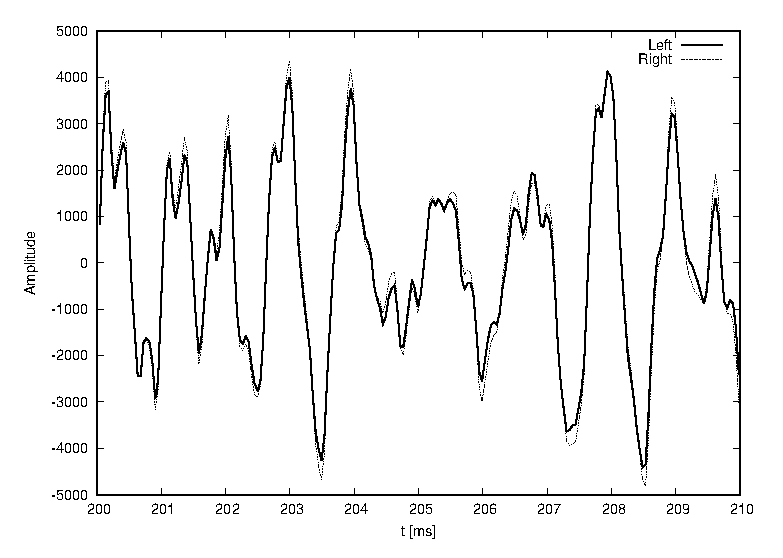
\includegraphics[width=0.8\hsize]{images/chimes.eps}
            \caption{chimes.wav}
            \label{fig:wav}
        \end{figure}

        図から, ほぼ同波形だが, 左右のデータが別々にサンプリングされていることがわかる.

\section{課題}
    $[0:2\pi)$の範囲を取る変数$\theta$について, 3種類の周期関数$f_i(\theta)$を考える.

    \begin{itemize}
        \item $\displaystyle f_1(\theta) = \frac{2}{\pi} \sum^M_{k = 1}\frac{\sin{k \theta}}{k}$
        \item $\displaystyle f_2(\theta) = \frac{4}{\pi} \sum^M_{k = 1}\frac{\sin{\{(2k - 1) \theta}\}}{2k - 1}$
        \item $\displaystyle f_3(\theta) = \frac{8}{\pi^2} \sum^M_{k = 1} \left(\sin{\frac{k\pi}{2}}\right) \frac{\sin{k\theta}}{k^2}$
    \end{itemize}

    それぞれの波形を振幅$A$, 周波数$f$ [Hz]の時系列データ$Af_i(t) + A_0$として生成するプログラム
    f1.c, f2.c, f3.cを一部抜粋してリスト\ref{src:f1}, \ref{src:f2}, \ref{src:f3}に示す.

    \begin{lstlisting}[caption=f1.c, label=src:f1]
#define BIAS 0x80
        
int main(int argc, char **argv) {
    int m, n, t;
    double amp, r, vin;
    unsigned char vout;

    for (t = 0; t <= 1000; t += 2) {
        for (vin = BIAS, n = 1; n <= m; n++) {
            r = (t * 2.0 / 1000.0 * 2.0 * PI) * n;
            vin += 2.0 * amp * sin(r) / (double)n / PI;
        }

        printf("%d, %4d\n", t, vout);
    }
}\end{lstlisting}

    \begin{lstlisting}[caption=f2.c, label=src:f2]
#define BIAS 0x80

int main(int argc, char **argv) {
    int m, n, t;
    double amp, r, vin;
    unsigned char vout;

    for (t = 0; t <= 1000; t += 2) {
        for (vin = BIAS, n = 1; n <= m; n++) {
            r = (t * 2.0 / 1000.0 * 2.0 * PI) * (2 * n - 1);
            vin += 4.0 * amp * sin(r) / (double)(2 * n - 1) / PI;
        }

        printf("%d, %4d\n", t, vout);
    }
}\end{lstlisting}

    \begin{lstlisting}[caption=f3.c, label=src:f3]
#define BIAS 0x80

int main(int argc, char **argv) {
    int m, n, t;
    double amp, r, vin;
    unsigned char vout;

    for (t = 0; t <= 1000; t += 2) {
        for (vin = BIAS, n = 1; n <= m; n++) {
            r = (t * 2.0 / 1000.0 * 2.0 * PI) * n;
            vin += 8.0 * amp * sin(r) / (double)n / (double)n / PI / PI * sin(n * PI / 2.0);
        }
        
        printf("%d, %4d\n", t, vout);
    }
}\end{lstlisting}

    これらのプログラムを使って, $A = 100, A_0 = 128, f = 2$ Hzとし, $M = 1, 10, 100$について波形を出力したものを
    図\ref{fig:f1}, \ref{fig:f2}, \ref{fig:f3}に示す.

    \begin{figure}[h]
        \centering
        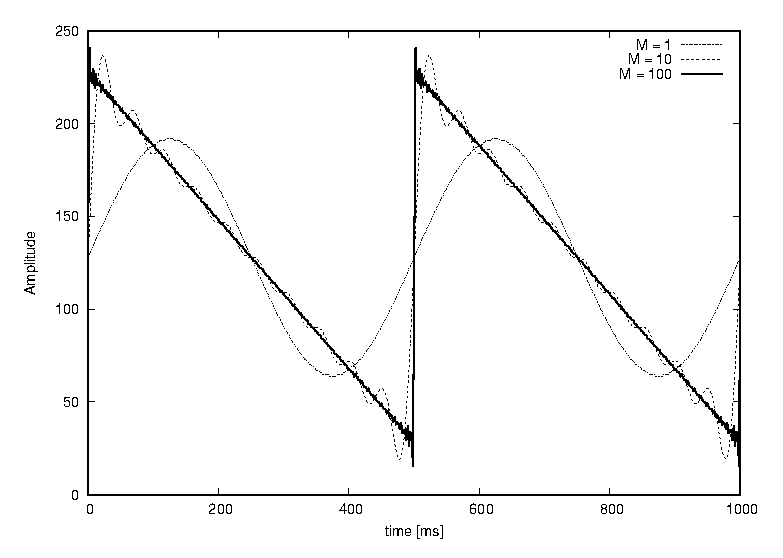
\includegraphics[width=0.8\hsize]{images/f1.eps}
        \caption{$f_1$の波形}
        \label{fig:f1}
    \end{figure}

    \begin{figure}[h]
        \centering
        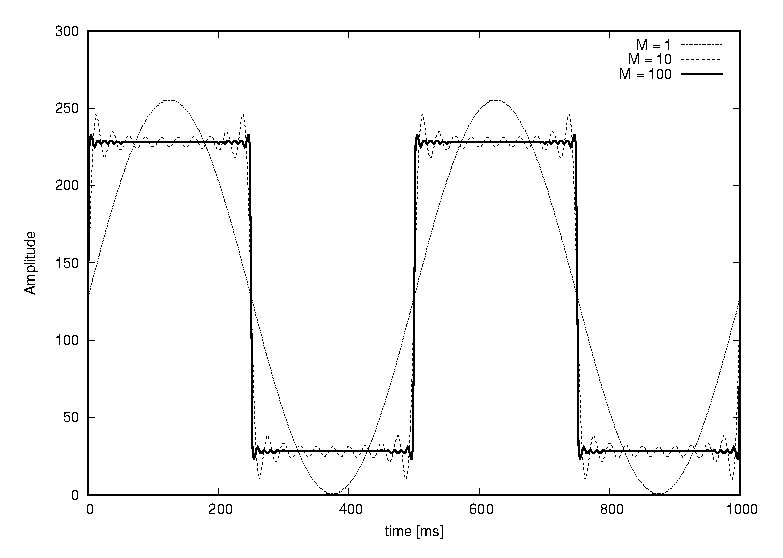
\includegraphics[width=0.8\hsize]{images/f2.eps}
        \caption{$f_2$の波形}
        \label{fig:f2}
    \end{figure}

    \begin{figure}[h]
        \centering
        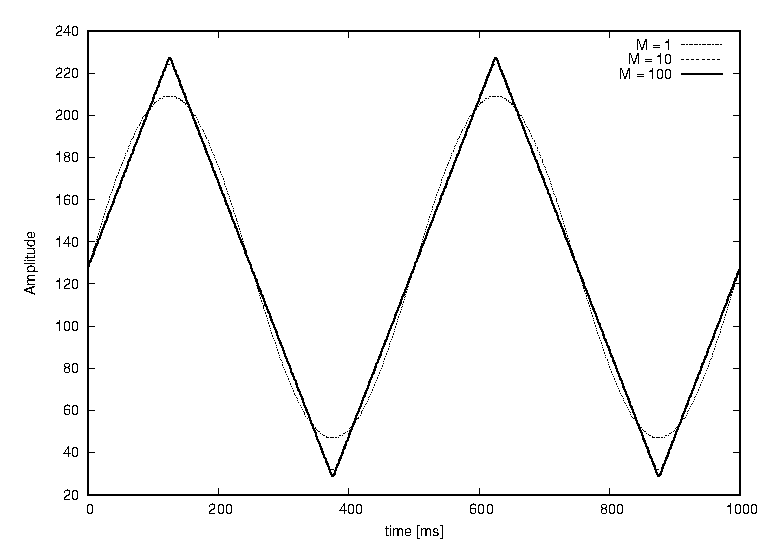
\includegraphics[width=0.8\hsize]{images/f3.eps}
        \caption{$f_3$の波形}
        \label{fig:f3}
    \end{figure}

    図より, それぞれ$M$が増加するほどのこぎり波, 矩形波, 三角波に近づいていることがわかる.

    次に, $M = 100$の場合のそれぞれの波形に, 演習3-1で実装したadd-wn2.cを使用して最大振幅10の
    白色雑音を加える. この波形を演習3-2, 3-3で実装したmvave3-1.c,
    mvave5-1.cを使用して雑音除去したものを図\ref{fig:f1mv}, \ref{fig:f2mv}, \ref{fig:f3mv}に示す.

    \begin{figure}[h]
        \centering
        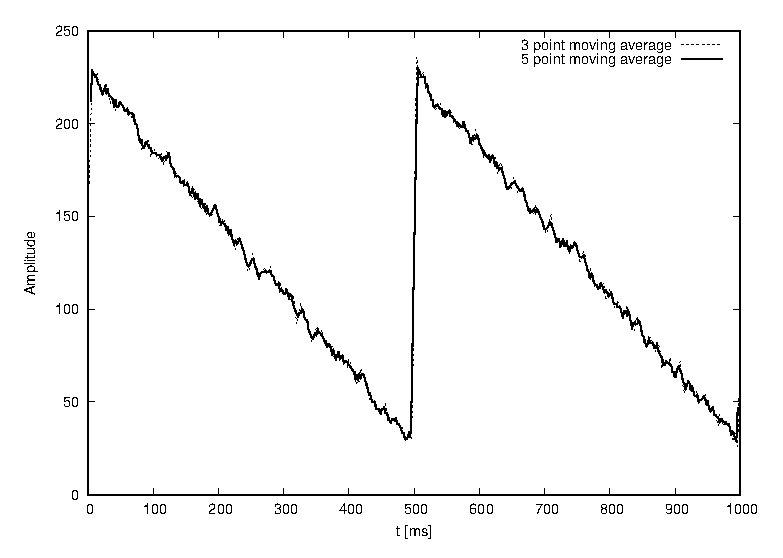
\includegraphics[width=0.8\hsize]{images/f1mv.eps}
        \caption{雑音を加え, 除去した$f_1$の波形}
        \label{fig:f1mv}
    \end{figure}

    \begin{figure}[h]
        \centering
        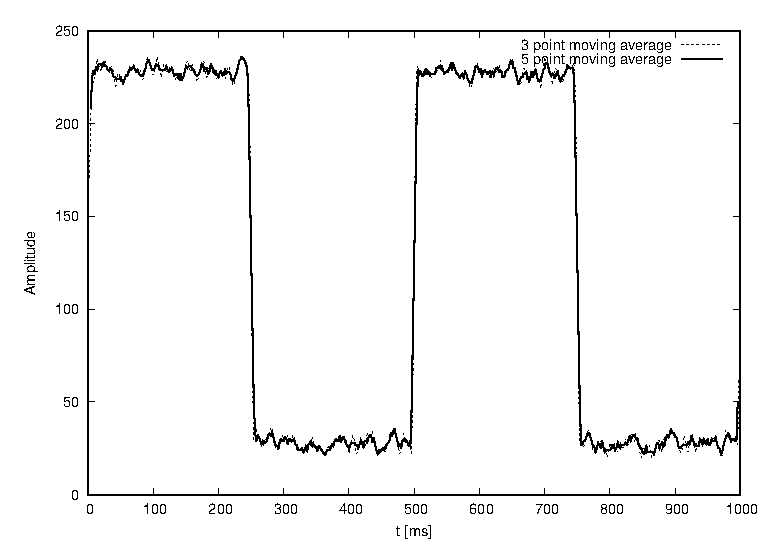
\includegraphics[width=0.8\hsize]{images/f2mv.eps}
        \caption{雑音を加え, 除去した$f_2$の波形}
        \label{fig:f2mv}
    \end{figure}

    \begin{figure}[h]
        \centering
        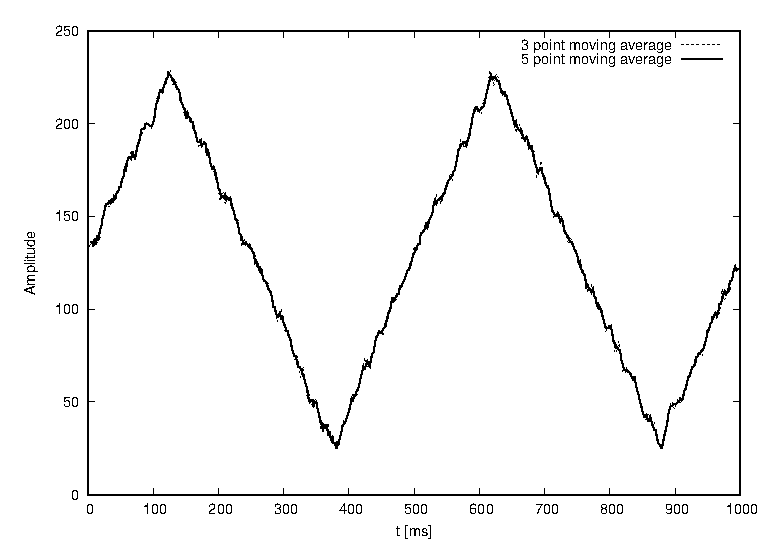
\includegraphics[width=0.8\hsize]{images/f3mv.eps}
        \caption{雑音を加え, 除去した$f_3$の波形}
        \label{fig:f3mv}
    \end{figure}

    また, これらの波形と雑音を加える前のそれぞれの波形のSNRを演習4-4で実装したsnr.cを使用して求め,
    表\ref{tab:fsnr}にまとめる.

    \begin{table}[h]
        \centering
        \caption{雑音を加え, 除去した波形と雑音を加える前の波形のSNR [dB]}
        \label{tab:fsnr}
        \begin{tabular}{c|ccc} \hline
            波形 & $f_1$ & $f_2$ & $f_3$ \\ \hline \hline
            3点移動平均 & 17.35 & 19.34 & 23.97 \\
            5点移動平均 & 14.46 & 15.69 & 23.22 \\ \hline
        \end{tabular}
    \end{table}

    これらの結果から, 演習4-4の結果と合わせて, 5点移動平均の方が雑音除去性能が優れているといえる.

\section{発展課題}

\section{感想および改善案}
    6月末に, 「まだ最終レポートまでは時間がたくさんあるな」などと思っていたが,
    気づけば8月になっていた.
    幸い演習は終わらせてあったため, あまり慌てることなく実験内容を復習しながらレポート作成に取り組めた.
    今回の実験を通して, gnuplotやコマンドライン引数など, 今後に役立てられるようなツールを使いこなせるようになり,
    とても良い経験ができたと思う.

    課題について, のこぎり波などのフーリエ級数を導出からする課題であればより楽しめたと思った.

\begin{thebibliography}{99}
    \bibitem{Support Page} Ec4電子制御工学実験 https://www2.st.nagaoka-ct.ac.jp/
    \bibitem{Text} 高橋章, 信号処理プログラミング, 令和2年$\cdot$前期
\end{thebibliography}

\end{document}
